% act_1.7
\subsection{Joint PD control $+$ gravity $+$ feed-forward term}
The objective of this activity is display the UR5 robot on rviz and control the motion of its joints with a PD with gravity compensation and a feed-forward term control method. The control is control method is given by $ \tau = M \ddot{q}_{\mathrm{des}} + k_p e + k_d \dot{e} + g$ where $M$ is the inertia matrix and $g$ is the gravitational effects vector. The simulation starts with the initial joint configuration $\begin{bmatrix} \pi & -\frac{\pi}{8} & -\frac{\pi}{6} & 0.0 & 0.0 & 0.0 \end{bmatrix}$ rad and then move the second and fifth joints of the UR5 robot. On one hand, the two joints will maintain the initial configuration during first $2$ seconds and follow a step reference during last $3$ seconds. On the other hand, the two joints will move following a sinusoidal trajectory during first $4$ seconds and maintain a constant joint position during last second. Finally, the performance of the control method will be evaluated in next subsections.

\subsubsection{Sinusoidal reference}
The Algorithm \ref{lst:joint_PD_gravity_feedforward_sin} control the movements of second and fifth joints of the UR5 robot to follow a sinusoidal reference trajectory. In this file, the PD with gravity compensation and a feed-forward term control method is configured with $K_p=300$ $\mathrm{\frac{N.m}{rad}}$ and $K_d=20$ $\mathrm{\frac{N.m.s}{rad}}$. Figure \ref{fig:act_1.7_sin_joint_position} shows the tracking performance of each joint of the UR5 robot. On one hand, the second joint ($\mathrm{q}_2$) presents position error at the beginning and final of the simulation but a good trajectory tracking from $1$ to $4$ seconds. The position error at the beginning is due to the reference speed starting with a value other than 0. Figure \ref{fig:act_1.7_sin_joint_velocity} shows the reference and measured velocity of each joint of UR5 robot. On the other hand, the fifth joint ($\mathrm{q}_5$) presents an excellent trajectory tracking except when reference trajectory change from sinusoidal to constant. The position error of $\mathrm{q}_5$ could be generated by the Coriolis and centripetal forces that has a high value when the reference trajectory change from sinusoidal to constant. Figure \ref{fig:act_1.7_sin_C} shows the value of Coriolis and centripetal forces for each joint and a red dot indicating the peak value.

\begin{lstlisting}[language=Python,caption={Move the second and fifth joint of UR5 robot with the requirement motion of activity 1.7.1}, label={lst:joint_PD_gravity_feedforward_sin}]
# =========================
#   Configuration of node
# =========================
# create a node: 
rospy.init_node("node_joint_PD_control_gravity_feedforward_term")

# public in topic /joint_states	to send joint data	
pub = rospy.Publisher('joint_states', JointState, queue_size=1000)

# loop rate (in Hz)
rate 	= rospy.Rate(1000)		# 100 [Hz]
dt 		= 1e-3					# 10  [ms]

# object(message) type JointState
jstate = JointState()

# ==========================================
#   Set initial joint configuration of UR5
# ==========================================
# initial configuration: position, velocity and acceleration 
q0 =   np.array([np.pi, -np.pi/8,  -np.pi/6, 0.0, 0.0, 0.0])
dq0 =  np.array([0.0, 0.0, 0.0, 0.0, 0.0, 0.0]) 
ddq0 = np.array([0.0, 0.0, 0.0, 0.0, 0.0, 0.0]) 

# desired trajectory: position, velocity and acceleration
q_des =   np.array([np.pi, -np.pi/8,  -np.pi/6, 0.0, 0.0, 0.0]) 
dq_des =  np.array([0.0, 0.0, 0.0, 0.0, 0.0, 0.0]) 
ddq_des = np.array([0.0, 0.0, 0.0, 0.0, 0.0, 0.0]) 

# measured trajectory: position, velocity and acceleration
q =   np.array([np.pi, -np.pi/8,  -np.pi/6, 0.0, 0.0, 0.0])
dq =  np.array([0.0, 0.0, 0.0, 0.0, 0.0, 0.0]) 
ddq = np.array([0.0, 0.0, 0.0, 0.0, 0.0, 0.0]) 

# ===========================
#   UR5 robot configuration
# ===========================
# joints name of UR5 robot
jnames = ['shoulder_pan_joint', 'shoulder_lift_joint', 'elbow_joint','wrist_1_joint', 'wrist_2_joint', 'wrist_3_joint']

# number of degress of freedom
ndof = 6
# the class robot load the ur5.urdf
ur5_robot = Robot(ndof,q0, dq0, dt)
# create inertia matrix 
M = np.zeros([ndof,ndof])
# create nonlinear effects vector
b = np.zeros(ndof)
# create gravity vector
g = np.zeros(ndof)

# ===============================
#   PD controller configuration
# ===============================
# proportional gain
kp = 300*np.ones(ndof)
# derivative gain
kd = 20*np.ones(ndof)
# control vector
tau = np.zeros(ndof)    

#===============
#   Simulation
#===============
t = 0.0             # [sec] 
sim_duration = 5.0  # [sec]
sine_duration = 4.0 # [sec]

while not rospy.is_shutdown():
    # generate sinusoidal joint reference
    if t<=sine_duration:
        # second link
        q_des[1], dq_des[1], ddq_des[1] = sinusoidal_reference_generator(q0[1], dq0[1], ddq0[1], 0.2, 1, t)
        last_q_des_1 = q_des[1]
        # fifth link
        q_des[4], dq_des[4], ddq_des[4] = sinusoidal_reference_generator(q0[4], dq0[4], ddq0[4], 0.4, 1.5, t)  
        last_q_des_4 = q_des[4]  
    else:   
        # second link
        q_des[1], dq_des[1], ddq_des[1] = step_reference_generator(0, last_q_des_1)
        # fifth link
        q_des[4], dq_des[4], ddq_des[4] = step_reference_generator(0 , last_q_des_4)
    
    # error: position and velocity
    e 	=  q_des - q
    de 	=  dq_des - dq    

    # compute inertia matrix
    M = ur5_robot.get_M()

    # compute gravitational effects vector
    g = ur5_robot.get_g()

    # PD control method + gravity compensation + feedforward term
    tau_ff = M.dot(ddq_des)
    tau = np.multiply(kp, e) + np.multiply(kd, de) + tau_ff + g
    
    # send control signal
    ur5_robot.send_control_command(tau)
    # update states
    q, dq, ddq = ur5_robot.read_joint_position_velocity_acceleration()

    # publish message
    jstate.header.stamp = rospy.Time.now()
    jstate.name 		= jnames			# Joints position name
    jstate.position 	= q
    jstate.velocity 	= dq
    pub.publish(jstate)

    # update time
    t = t + dt

    # stop simulation
    if t>=sim_duration:
        print("stopping rviz ...")
        break
    rate.sleep()
\end{lstlisting}
 
\begin{figure}[H]
	\centering
	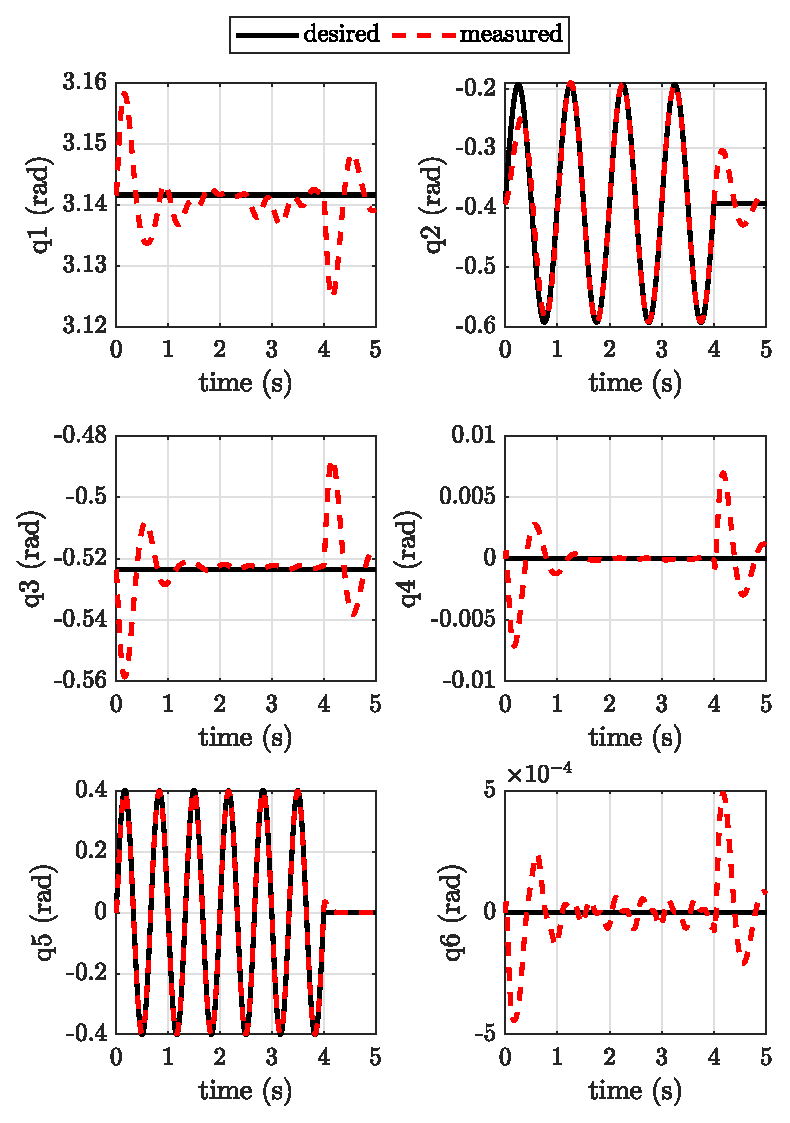
\includegraphics{images/act_1.7_sin/joint_position.eps}
	\caption{Angular position of each joint of UR5 robot with Algorithm \ref{lst:joint_PD_gravity_feedforward_sin}.}
	\label{fig:act_1.7_sin_joint_position}
\end{figure}
 
\begin{figure}[H]
	\centering
	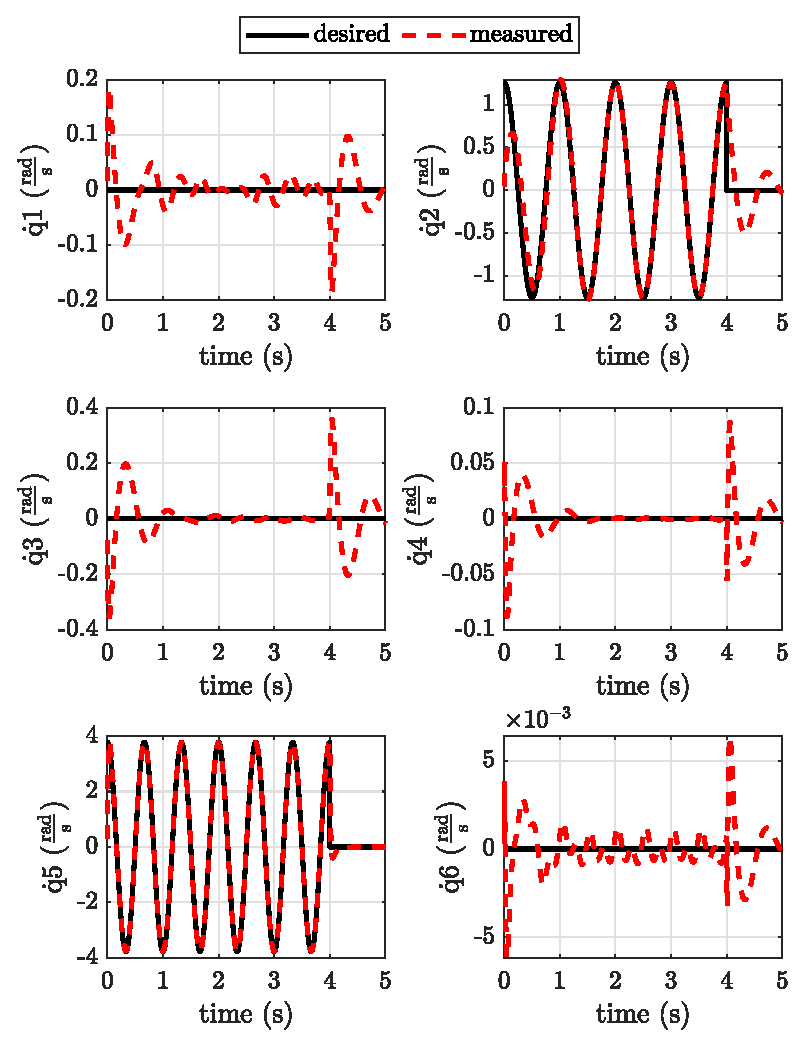
\includegraphics{images/act_1.7_sin/joint_velocity.eps}
	\caption{Angular velocity of each joint of UR5 robot with Algorithm \ref{lst:joint_PD_gravity_feedforward_sin}.}
	\label{fig:act_1.7_sin_joint_velocity}
\end{figure} 

\begin{figure}[H]
	\centering
	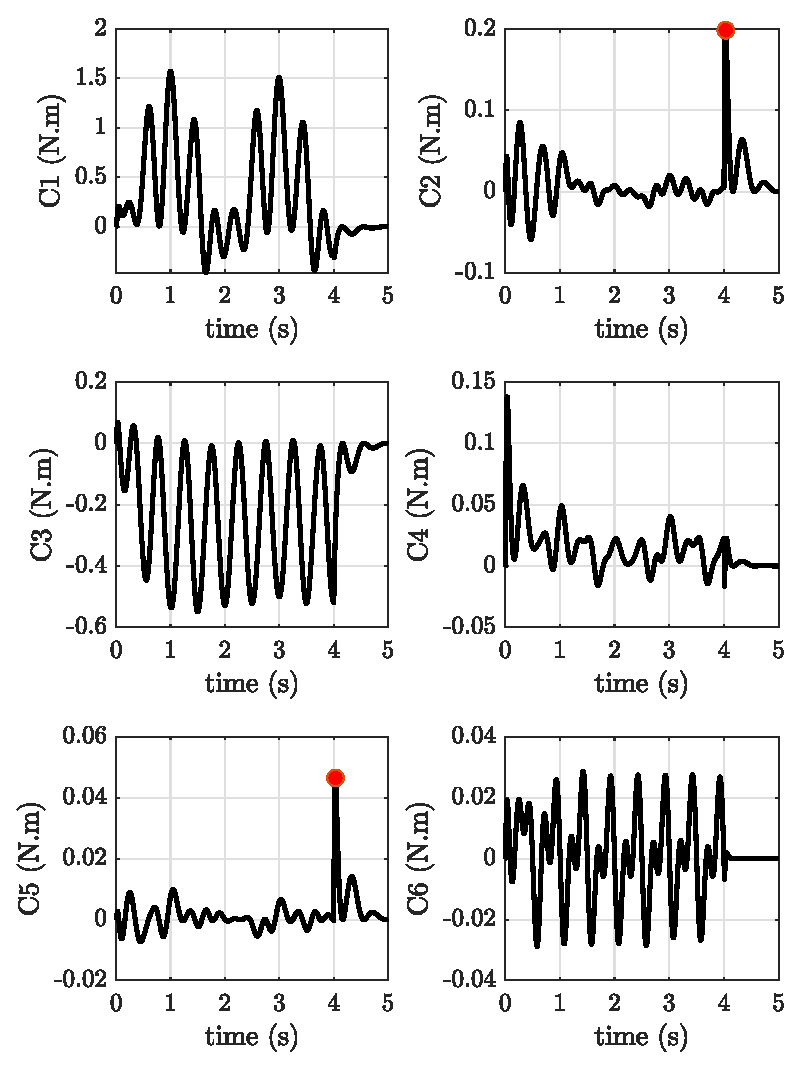
\includegraphics{images/act_1.7_sin/C.eps}
	\caption{Coriolis and centripetal forces ($C$). The red dot indicates the peak value of $C$ when the reference trajectory change form sinusoidal to constant.}
	\label{fig:act_1.7_sin_C}
\end{figure} 

\newpage
\subsubsection{Step reference}
The Algorithm \ref{lst:joint_PD_gravity_feedforward_step} control the movements of second and fifth joints of the UR5 robot to follow a step reference trajectory. In this file, the PD with gravity compensation and a feed-forward term control method is configured with $K_p=300$ $\mathrm{\frac{N.m}{rad}}$ and $K_d=20$ $\mathrm{\frac{N.m.s}{rad}}$. Figure \ref{fig:act_1.7_step_joint_position} shows the tracking performance of each joint of the UR5 robot. In this case, the performance of the new control method is same as PD with gravity compensation due to desired acceleration is $0$ $\mathrm{\frac{rad}{s^2}}$, so feed-forward term is $0$. \vspace{5px}

\begin{lstlisting}[language=Python,caption={Move the second and fifth joint of UR5 robot with the requirement motion of activity 1.7.2}, label={lst:joint_PD_gravity_feedforward_step}]
# =========================
#   Configuration of node
# =========================
# create a node: 
rospy.init_node("node_joint_PD_control_gravity_compensation_feed_forward_term")

# public in topic /joint_states	to send joint data	
pub = rospy.Publisher('joint_states', JointState, queue_size=1000)

# loop rate (in Hz)
rate 	= rospy.Rate(1000)		# 100 [Hz]
dt 		= 1e-3					# 10  [ms]

# object(message) type JointState
jstate = JointState()

# ==========================================
#   Set initial joint configuration of UR5
# ==========================================
# initial configuration: position, velocity and acceleration 
q0 =   np.array([np.pi, -np.pi/8,  -np.pi/6, 0.0, 0.0, 0.0])
dq0 =  np.array([0.0, 0.0, 0.0, 0.0, 0.0, 0.0]) 
ddq0 = np.array([0.0, 0.0, 0.0, 0.0, 0.0, 0.0]) 

# desired trajectory: position, velocity and acceleration
q_des =   np.array([np.pi, -np.pi/8,  -np.pi/6, 0.0, 0.0, 0.0]) 
dq_des =  np.array([0.0, 0.0, 0.0, 0.0, 0.0, 0.0]) 
ddq_des = np.array([0.0, 0.0, 0.0, 0.0, 0.0, 0.0]) 

# measured trajectory: position, velocity and acceleration
q =   np.array([np.pi, -np.pi/8,  -np.pi/6, 0.0, 0.0, 0.0])
dq =  np.array([0.0, 0.0, 0.0, 0.0, 0.0, 0.0]) 
ddq = np.array([0.0, 0.0, 0.0, 0.0, 0.0, 0.0]) 

# ===========================
#   UR5 robot configuration
# ===========================
# joints name of UR5 robot
jnames = ['shoulder_pan_joint', 'shoulder_lift_joint', 'elbow_joint','wrist_1_joint', 'wrist_2_joint', 'wrist_3_joint']

# number of degress of freedom
ndof = 6
# the class robot load the ur5.urdf
ur5_robot = Robot(ndof,q0, dq0, dt)
# create inertia matrix 
M = np.zeros([ndof,ndof])
# create nonlinear effects vector
b = np.zeros(ndof)
# create gravity vector
g = np.zeros(ndof)

# ===============================
#   PD controller configuration
# ===============================
# proportional gain
kp = 300*np.ones(ndof)
# derivative gain
kd = 20*np.ones(ndof)
# control vector
tau = np.zeros(ndof)    

#===============
#   Simulation
#===============
t = 0.0             # [sec] 
sim_duration = 5.0  # [sec]
step_start = 2.0    # [sec]

while not rospy.is_shutdown():
    # generate step reference after 2 seconds
    if t>=step_start:
        # second link
        q_des[1], dq_des[1], ddq_des[1] = step_reference_generator(q0[1], -0.4)
        # fifth link
        q_des[4], dq_des[4], ddq_des[4] = step_reference_generator(q0[4], 0.5)

    # error: position and velocity
    e 	=  q_des - q
    de 	=  dq_des - dq    
    
    # compute inertia matrix
    M = ur5_robot.get_M()

    # compute gravitational effects vector
    g = ur5_robot.get_g()

    # Coriolis and centripetal forces
    C = ur5_robot.get_b() - g

    # PD control method + gravity compensation + feedforward term
    tau_ff = M.dot(ddq_des)
    tau = np.multiply(kp, e) + np.multiply(kd, de) + tau_ff + g
    
    # send control signal
    ur5_robot.send_control_command(tau)
    # update states
    q, dq, ddq = ur5_robot.read_joint_position_velocity_acceleration()

    # publish message
    jstate.header.stamp = rospy.Time.now()
    jstate.name 		= jnames			# Joints position name
    jstate.position 	= q
    jstate.velocity 	= dq
    pub.publish(jstate)

    # update time
    t = t + dt
   
    # stop simulation
    if t>=sim_duration:
        print("stopping rviz ...")
        break
    rate.sleep()
\end{lstlisting}

\begin{figure}[H]
	\centering
	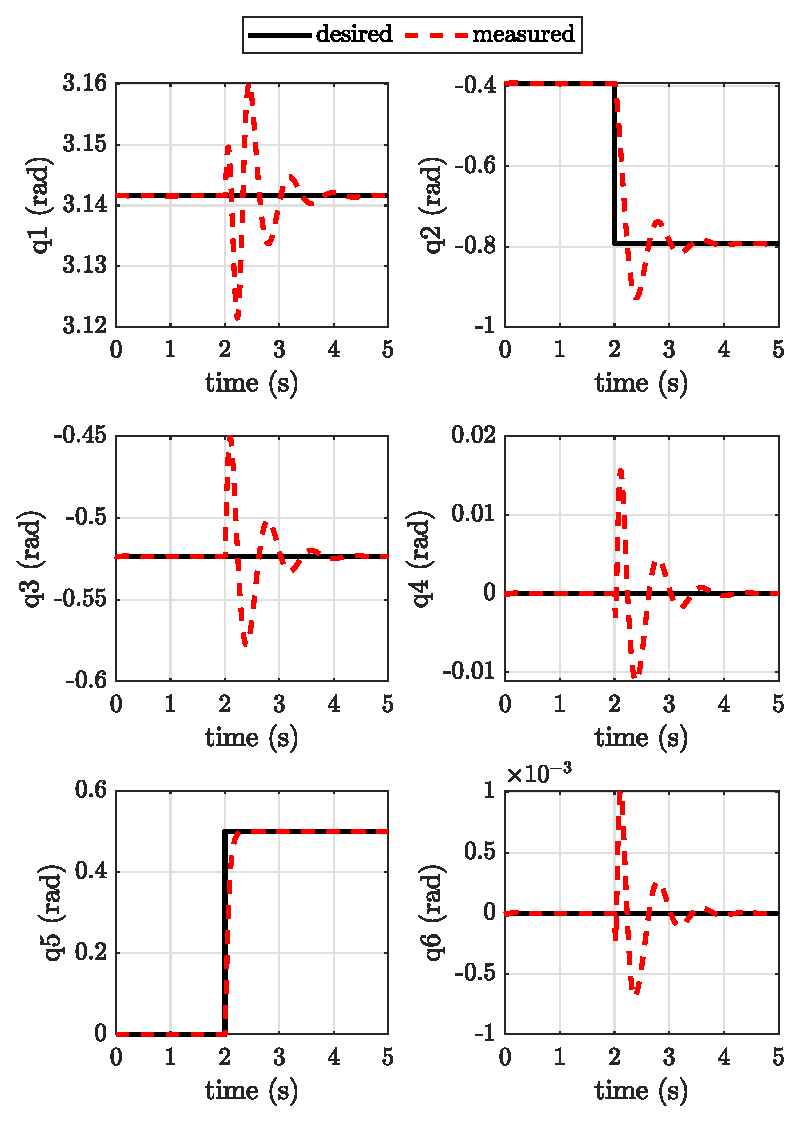
\includegraphics{images/act_1.7_step/joint_position.eps}
	\caption{Angular position of each joint of UR5 robot with Algorithm \ref{lst:joint_PD_gravity_feedforward_step}.}
	\label{fig:act_1.7_step_joint_position}
\end{figure}
